\section{Results}
As stated previously, each algorithm has been applied to the MNIST and ORL datasets. It is important to know that the MNIST dataset comes already split in training data (60000 samples) and test data (10000 samples), whereas the ORL dataset had to be manually and randomly split in 70\% training samples and 30\% test samples.

The MNIST dataset is composed of 70000 pictures of handwritten digits in grayscale, from 0 to 9, and with an image resolution of 28x28.
\begin{figure}
  \centering
      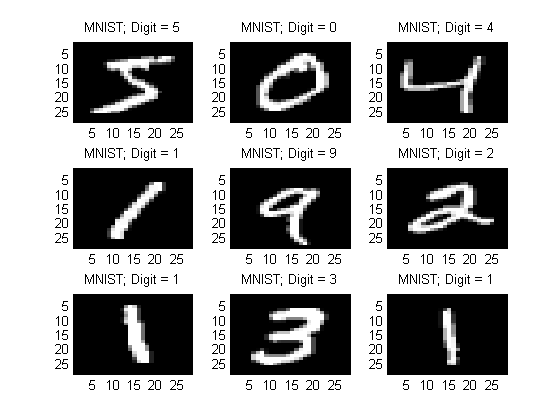
\includegraphics[width=0.5\textwidth]{fig/mnist_example.png}
  \caption{MNIST dataset sample}
\end{figure}

 The ORL dataset consists of 400 facial pictures, for it contains 10 pictures for each of the 40 persons, thus giving 40 classes.
\begin{figure}
  \centering
  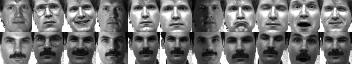
\includegraphics[width=0.4\textwidth]{fig/orl.jpg}
  \caption{ORL dataset sample}
\end{figure}

Each algorithm has been compared by execution time, and success rate (or accuracy). It can be seen that changing the hyperparameters of one can drastically improve its success rate, as the Nearest Sub-class Centroid Classifier shows for instance, with the given hyperparameters \{2,3,5\} corresponding to the number of sub-classes. The learning rate for the backpropagation algorithm has been set to 0.1, after experimentation and fine-tuning.
\\

INSERT MNIST SUCCESS RATE
\\

INSERT ORL SUCCESS RATE
\\

The bar diagrams showed in figure 3 and 4 clearly show that ...


